% Created by tikzDevice version 0.6.2-92-0ad2792 on 2013-11-12 07:52:59
% !TEX encoding = UTF-8 Unicode
\documentclass[12pt, mainfont = Minion,     mainscale = 1.0, sansfont = Myriad,     sansscale = MatchLowercase, monofont = Consolas,   monoscale = MatchLowercase, mathfont = MinionMath, mathscale = 1.0]{mtikzfig}
\begin{document}

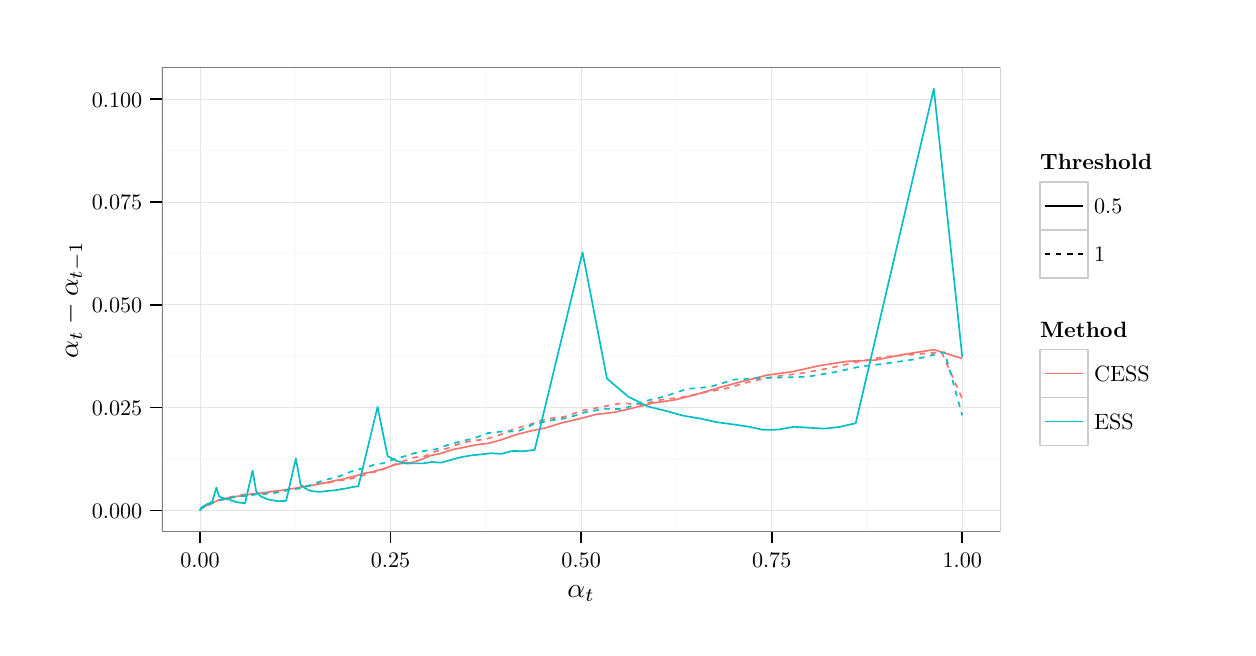
\begin{tikzpicture}[x=1pt,y=1pt]
\definecolor[named]{fillColor}{rgb}{1.00,1.00,1.00}
\path[use as bounding box,fill=fillColor,fill opacity=0.00] (0,0) rectangle (433.62,216.81);
\begin{scope}
\path[clip] (  0.00,  0.00) rectangle (433.62,216.81);
\definecolor[named]{drawColor}{rgb}{1.00,1.00,1.00}
\definecolor[named]{fillColor}{rgb}{1.00,1.00,1.00}

\path[draw=drawColor,line width= 0.6pt,line join=round,line cap=round,fill=fillColor] (  0.00,  0.00) rectangle (433.62,216.81);
\end{scope}
\begin{scope}
\path[clip] ( 48.51, 34.74) rectangle (351.48,202.36);
\definecolor[named]{fillColor}{rgb}{1.00,1.00,1.00}

\path[fill=fillColor] ( 48.51, 34.74) rectangle (351.48,202.36);
\definecolor[named]{drawColor}{rgb}{0.98,0.98,0.98}

\path[draw=drawColor,line width= 0.6pt,line join=round] ( 48.51, 60.94) --
	(351.48, 60.94);

\path[draw=drawColor,line width= 0.6pt,line join=round] ( 48.51, 98.11) --
	(351.48, 98.11);

\path[draw=drawColor,line width= 0.6pt,line join=round] ( 48.51,135.28) --
	(351.48,135.28);

\path[draw=drawColor,line width= 0.6pt,line join=round] ( 48.51,172.44) --
	(351.48,172.44);

\path[draw=drawColor,line width= 0.6pt,line join=round] ( 96.71, 34.74) --
	( 96.71,202.36);

\path[draw=drawColor,line width= 0.6pt,line join=round] (165.57, 34.74) --
	(165.57,202.36);

\path[draw=drawColor,line width= 0.6pt,line join=round] (234.42, 34.74) --
	(234.42,202.36);

\path[draw=drawColor,line width= 0.6pt,line join=round] (303.28, 34.74) --
	(303.28,202.36);
\definecolor[named]{drawColor}{rgb}{0.90,0.90,0.90}

\path[draw=drawColor,line width= 0.2pt,line join=round] ( 48.51, 42.36) --
	(351.48, 42.36);

\path[draw=drawColor,line width= 0.2pt,line join=round] ( 48.51, 79.53) --
	(351.48, 79.53);

\path[draw=drawColor,line width= 0.2pt,line join=round] ( 48.51,116.69) --
	(351.48,116.69);

\path[draw=drawColor,line width= 0.2pt,line join=round] ( 48.51,153.86) --
	(351.48,153.86);

\path[draw=drawColor,line width= 0.2pt,line join=round] ( 48.51,191.03) --
	(351.48,191.03);

\path[draw=drawColor,line width= 0.2pt,line join=round] ( 62.28, 34.74) --
	( 62.28,202.36);

\path[draw=drawColor,line width= 0.2pt,line join=round] (131.14, 34.74) --
	(131.14,202.36);

\path[draw=drawColor,line width= 0.2pt,line join=round] (200.00, 34.74) --
	(200.00,202.36);

\path[draw=drawColor,line width= 0.2pt,line join=round] (268.85, 34.74) --
	(268.85,202.36);

\path[draw=drawColor,line width= 0.2pt,line join=round] (337.71, 34.74) --
	(337.71,202.36);
\definecolor[named]{drawColor}{rgb}{0.97,0.46,0.43}

\path[draw=drawColor,line width= 0.6pt,line join=round] ( 62.28, 42.36) --
	( 62.28, 42.37) --
	( 62.28, 42.37) --
	( 62.29, 42.37) --
	( 62.29, 42.37) --
	( 62.29, 42.38) --
	( 62.30, 42.38) --
	( 62.31, 42.40) --
	( 62.32, 42.42) --
	( 62.33, 42.44) --
	( 62.35, 42.47) --
	( 62.38, 42.51) --
	( 62.42, 42.56) --
	( 62.47, 42.64) --
	( 62.54, 42.77) --
	( 62.63, 42.84) --
	( 62.75, 43.01) --
	( 62.89, 43.10) --
	( 63.04, 43.20) --
	( 63.23, 43.38) --
	( 63.42, 43.37) --
	( 63.64, 43.56) --
	( 63.90, 43.72) --
	( 64.20, 44.01) --
	( 64.53, 44.13) --
	( 64.88, 44.23) --
	( 65.23, 44.28) --
	( 65.65, 44.61) --
	( 66.09, 44.74) --
	( 66.57, 44.96) --
	( 67.12, 45.34) --
	( 67.71, 45.52) --
	( 68.34, 45.76) --
	( 69.03, 46.12) --
	( 69.76, 46.29) --
	( 70.54, 46.55) --
	( 71.34, 46.68) --
	( 72.17, 46.84) --
	( 73.00, 46.85) --
	( 73.86, 47.02) --
	( 74.77, 47.25) --
	( 75.71, 47.45) --
	( 76.68, 47.62) --
	( 77.67, 47.69) --
	( 78.70, 47.90) --
	( 79.76, 48.11) --
	( 80.86, 48.28) --
	( 81.96, 48.27) --
	( 83.11, 48.60) --
	( 84.27, 48.63) --
	( 85.45, 48.74) --
	( 86.67, 48.93) --
	( 87.93, 49.17) --
	( 89.23, 49.34) --
	( 90.55, 49.48) --
	( 91.89, 49.61) --
	( 93.28, 49.89) --
	( 94.73, 50.15) --
	( 96.20, 50.30) --
	( 97.71, 50.55) --
	( 99.30, 50.90) --
	(100.93, 51.18) --
	(102.60, 51.38) --
	(104.34, 51.73) --
	(106.13, 52.07) --
	(108.00, 52.43) --
	(109.95, 52.88) --
	(111.98, 53.33) --
	(114.08, 53.67) --
	(116.29, 54.32) --
	(118.60, 54.81) --
	(121.07, 55.68) --
	(123.61, 56.12) --
	(126.29, 56.79) --
	(129.10, 57.53) --
	(132.12, 58.67) --
	(135.27, 59.39) --
	(138.47, 59.59) --
	(141.85, 60.60) --
	(145.51, 62.15) --
	(149.33, 62.97) --
	(153.40, 64.32) --
	(157.62, 65.15) --
	(162.02, 66.08) --
	(166.51, 66.62) --
	(171.24, 67.91) --
	(176.31, 69.71) --
	(181.63, 71.06) --
	(187.15, 72.19) --
	(193.02, 74.01) --
	(199.14, 75.44) --
	(205.58, 77.09) --
	(212.15, 77.85) --
	(219.03, 79.45) --
	(226.23, 81.23) --
	(233.62, 82.27) --
	(241.37, 84.21) --
	(249.58, 86.66) --
	(258.22, 88.98) --
	(267.28, 91.26) --
	(276.57, 92.54) --
	(286.27, 94.71) --
	(296.26, 96.25) --
	(306.32, 96.69) --
	(316.78, 98.80) --
	(327.54,100.44) --
	(337.71, 97.26);

\path[draw=drawColor,line width= 0.6pt,dash pattern=on 2pt off 2pt ,line join=round] ( 62.28, 42.36) --
	( 62.28, 42.37) --
	( 62.28, 42.37) --
	( 62.29, 42.37) --
	( 62.29, 42.37) --
	( 62.29, 42.38) --
	( 62.30, 42.40) --
	( 62.31, 42.41) --
	( 62.32, 42.44) --
	( 62.34, 42.45) --
	( 62.36, 42.48) --
	( 62.40, 42.56) --
	( 62.45, 42.61) --
	( 62.51, 42.68) --
	( 62.58, 42.76) --
	( 62.69, 42.94) --
	( 62.81, 43.03) --
	( 62.96, 43.16) --
	( 63.13, 43.29) --
	( 63.33, 43.44) --
	( 63.55, 43.56) --
	( 63.79, 43.66) --
	( 64.06, 43.80) --
	( 64.36, 43.98) --
	( 64.68, 44.10) --
	( 65.03, 44.25) --
	( 65.42, 44.44) --
	( 65.81, 44.49) --
	( 66.28, 44.85) --
	( 66.78, 45.11) --
	( 67.33, 45.33) --
	( 67.93, 45.56) --
	( 68.58, 45.89) --
	( 69.29, 46.20) --
	( 70.01, 46.20) --
	( 70.76, 46.42) --
	( 71.54, 46.59) --
	( 72.41, 47.05) --
	( 73.32, 47.29) --
	( 74.26, 47.40) --
	( 75.21, 47.49) --
	( 76.21, 47.77) --
	( 77.24, 47.94) --
	( 78.32, 48.16) --
	( 79.42, 48.28) --
	( 80.49, 48.18) --
	( 81.60, 48.31) --
	( 82.72, 48.40) --
	( 83.87, 48.62) --
	( 85.05, 48.68) --
	( 86.25, 48.85) --
	( 87.47, 48.96) --
	( 88.71, 49.05) --
	( 89.99, 49.24) --
	( 91.30, 49.43) --
	( 92.62, 49.51) --
	( 93.99, 49.77) --
	( 95.40, 49.95) --
	( 96.86, 50.23) --
	( 98.39, 50.62) --
	( 99.97, 50.91) --
	(101.62, 51.23) --
	(103.37, 51.83) --
	(105.18, 52.13) --
	(107.00, 52.19) --
	(108.86, 52.39) --
	(110.81, 52.89) --
	(112.81, 53.18) --
	(114.86, 53.40) --
	(116.99, 53.85) --
	(119.23, 54.48) --
	(121.60, 55.16) --
	(124.14, 56.05) --
	(126.77, 56.53) --
	(129.64, 57.85) --
	(132.73, 59.06) --
	(136.04, 60.24) --
	(139.59, 61.49) --
	(143.21, 61.90) --
	(147.14, 63.58) --
	(151.28, 64.71) --
	(155.72, 66.32) --
	(160.38, 67.54) --
	(165.14, 68.03) --
	(170.16, 69.49) --
	(175.60, 71.73) --
	(181.35, 73.39) --
	(187.48, 75.46) --
	(193.75, 76.16) --
	(200.43, 78.44) --
	(207.37, 79.80) --
	(214.54, 81.09) --
	(221.65, 80.69) --
	(229.06, 82.37) --
	(236.64, 83.29) --
	(244.54, 84.98) --
	(252.72, 86.52) --
	(261.36, 89.00) --
	(270.33, 90.79) --
	(279.51, 91.90) --
	(289.01, 93.64) --
	(298.91, 95.83) --
	(309.19, 97.86) --
	(319.63, 98.66) --
	(330.22, 99.58) --
	(337.71, 82.75);
\definecolor[named]{drawColor}{rgb}{0.00,0.75,0.77}

\path[draw=drawColor,line width= 0.6pt,line join=round] ( 62.28, 42.36) --
	( 62.29, 42.38) --
	( 62.30, 42.42) --
	( 62.31, 42.45) --
	( 62.34, 42.49) --
	( 62.39, 42.67) --
	( 62.49, 42.89) --
	( 62.63, 43.10) --
	( 62.82, 43.40) --
	( 63.05, 43.58) --
	( 63.30, 43.72) --
	( 63.60, 43.98) --
	( 63.90, 44.01) --
	( 64.25, 44.23) --
	( 64.65, 44.52) --
	( 65.10, 44.77) --
	( 65.56, 44.88) --
	( 66.11, 45.32) --
	( 66.65, 45.28) --
	( 68.19, 50.65) --
	( 69.14, 47.50) --
	( 70.02, 47.10) --
	( 70.83, 46.73) --
	( 71.60, 46.52) --
	( 72.35, 46.41) --
	( 73.07, 46.26) --
	( 73.72, 45.86) --
	( 74.36, 45.83) --
	( 74.94, 45.50) --
	( 75.50, 45.35) --
	( 76.04, 45.28) --
	( 76.56, 45.17) --
	( 77.08, 45.14) --
	( 77.58, 45.06) --
	( 78.08, 45.06) --
	( 78.58, 45.06) --
	( 81.25, 56.79) --
	( 82.55, 49.38) --
	( 83.61, 48.04) --
	( 84.52, 47.28) --
	( 85.37, 46.95) --
	( 86.15, 46.59) --
	( 86.89, 46.37) --
	( 87.60, 46.19) --
	( 88.29, 46.08) --
	( 88.96, 45.97) --
	( 89.61, 45.86) --
	( 90.24, 45.75) --
	( 90.86, 45.72) --
	( 91.49, 45.75) --
	( 92.13, 45.79) --
	( 92.76, 45.79) --
	( 93.42, 45.90) --
	( 96.90, 61.14) --
	( 98.63, 51.71) --
	(100.13, 50.47) --
	(101.49, 49.71) --
	(102.78, 49.31) --
	(104.05, 49.20) --
	(105.29, 49.09) --
	(106.56, 49.17) --
	(107.85, 49.35) --
	(109.17, 49.49) --
	(110.51, 49.57) --
	(111.88, 49.78) --
	(113.31, 50.07) --
	(114.77, 50.25) --
	(116.30, 50.58) --
	(117.88, 50.91) --
	(119.50, 51.09) --
	(126.43, 79.76) --
	(130.06, 61.98) --
	(133.37, 60.23) --
	(136.51, 59.33) --
	(139.67, 59.37) --
	(142.82, 59.37) --
	(146.06, 59.87) --
	(149.26, 59.62) --
	(152.62, 60.53) --
	(156.17, 61.51) --
	(159.84, 62.20) --
	(163.59, 62.59) --
	(167.42, 63.03) --
	(171.21, 62.81) --
	(175.20, 63.87) --
	(179.16, 63.76) --
	(183.21, 64.23) --
	(200.50,135.65) --
	(209.32, 90.00) --
	(216.95, 83.54) --
	(223.92, 79.98) --
	(230.59, 78.35) --
	(236.93, 76.60) --
	(243.08, 75.55) --
	(248.99, 74.25) --
	(254.75, 73.48) --
	(260.36, 72.65) --
	(265.76, 71.49) --
	(271.17, 71.56) --
	(276.77, 72.58) --
	(282.31, 72.25) --
	(287.78, 71.92) --
	(293.37, 72.54) --
	(299.21, 73.88) --
	(327.44,194.74) --
	(337.71, 97.76);

\path[draw=drawColor,line width= 0.6pt,dash pattern=on 2pt off 2pt ,line join=round] ( 62.28, 42.36) --
	( 62.28, 42.37) --
	( 62.28, 42.37) --
	( 62.29, 42.37) --
	( 62.29, 42.37) --
	( 62.29, 42.38) --
	( 62.30, 42.39) --
	( 62.31, 42.40) --
	( 62.32, 42.42) --
	( 62.33, 42.44) --
	( 62.35, 42.46) --
	( 62.37, 42.48) --
	( 62.40, 42.53) --
	( 62.44, 42.57) --
	( 62.50, 42.66) --
	( 62.58, 42.78) --
	( 62.66, 42.83) --
	( 62.77, 42.93) --
	( 62.91, 43.15) --
	( 63.10, 43.35) --
	( 63.27, 43.29) --
	( 63.47, 43.44) --
	( 63.72, 43.70) --
	( 63.97, 43.74) --
	( 64.25, 43.84) --
	( 64.57, 44.10) --
	( 64.91, 44.20) --
	( 65.27, 44.32) --
	( 65.69, 44.63) --
	( 66.14, 44.79) --
	( 66.64, 45.03) --
	( 67.18, 45.29) --
	( 67.74, 45.40) --
	( 68.36, 45.69) --
	( 69.01, 45.90) --
	( 69.72, 46.18) --
	( 70.45, 46.30) --
	( 71.18, 46.29) --
	( 71.93, 46.41) --
	( 72.71, 46.55) --
	( 73.55, 46.91) --
	( 74.44, 47.16) --
	( 75.35, 47.27) --
	( 76.25, 47.24) --
	( 77.21, 47.55) --
	( 78.18, 47.58) --
	( 79.16, 47.63) --
	( 80.14, 47.70) --
	( 81.16, 47.84) --
	( 82.23, 48.15) --
	( 83.32, 48.25) --
	( 84.41, 48.24) --
	( 85.51, 48.27) --
	( 86.64, 48.46) --
	( 87.77, 48.50) --
	( 88.94, 48.65) --
	( 90.15, 48.87) --
	( 91.40, 49.14) --
	( 92.70, 49.36) --
	( 94.06, 49.72) --
	( 95.47, 49.98) --
	( 96.92, 50.14) --
	( 98.39, 50.32) --
	( 99.94, 50.75) --
	(101.61, 51.33) --
	(103.40, 52.04) --
	(105.31, 52.67) --
	(107.35, 53.36) --
	(109.48, 53.86) --
	(111.71, 54.42) --
	(114.09, 55.22) --
	(116.69, 56.36) --
	(119.43, 57.16) --
	(122.28, 57.77) --
	(125.36, 58.99) --
	(128.52, 59.42) --
	(131.92, 60.70) --
	(135.51, 61.72) --
	(139.32, 62.93) --
	(143.31, 63.88) --
	(147.40, 64.45) --
	(151.78, 66.00) --
	(156.40, 67.30) --
	(161.23, 68.44) --
	(166.41, 70.33) --
	(171.70, 70.92) --
	(176.98, 70.84) --
	(182.75, 73.52) --
	(188.77, 74.85) --
	(194.96, 75.76) --
	(201.53, 77.85) --
	(208.33, 79.06) --
	(215.12, 79.00) --
	(222.41, 81.70) --
	(230.04, 83.53) --
	(238.17, 86.27) --
	(246.43, 86.96) --
	(255.19, 89.62) --
	(264.06, 90.23) --
	(272.95, 90.38) --
	(281.91, 90.70) --
	(291.15, 92.25) --
	(300.78, 94.33) --
	(310.63, 95.52) --
	(320.75, 97.01) --
	(331.35, 99.55) --
	(337.71, 76.68);
\definecolor[named]{drawColor}{rgb}{0.50,0.50,0.50}

\path[draw=drawColor,line width= 0.6pt,line join=round,line cap=round] ( 48.51, 34.74) rectangle (351.48,202.36);
\end{scope}
\begin{scope}
\path[clip] (  0.00,  0.00) rectangle (433.62,216.81);
\definecolor[named]{drawColor}{rgb}{0.00,0.00,0.00}

\node[text=drawColor,anchor=base east,inner sep=0pt, outer sep=0pt, scale=  0.80] at ( 41.40, 39.43) {0.000};

\node[text=drawColor,anchor=base east,inner sep=0pt, outer sep=0pt, scale=  0.80] at ( 41.40, 76.60) {0.025};

\node[text=drawColor,anchor=base east,inner sep=0pt, outer sep=0pt, scale=  0.80] at ( 41.40,113.77) {0.050};

\node[text=drawColor,anchor=base east,inner sep=0pt, outer sep=0pt, scale=  0.80] at ( 41.40,150.93) {0.075};

\node[text=drawColor,anchor=base east,inner sep=0pt, outer sep=0pt, scale=  0.80] at ( 41.40,188.10) {0.100};
\end{scope}
\begin{scope}
\path[clip] (  0.00,  0.00) rectangle (433.62,216.81);
\definecolor[named]{drawColor}{rgb}{0.00,0.00,0.00}

\path[draw=drawColor,line width= 0.6pt,line join=round] ( 44.24, 42.36) --
	( 48.51, 42.36);

\path[draw=drawColor,line width= 0.6pt,line join=round] ( 44.24, 79.53) --
	( 48.51, 79.53);

\path[draw=drawColor,line width= 0.6pt,line join=round] ( 44.24,116.69) --
	( 48.51,116.69);

\path[draw=drawColor,line width= 0.6pt,line join=round] ( 44.24,153.86) --
	( 48.51,153.86);

\path[draw=drawColor,line width= 0.6pt,line join=round] ( 44.24,191.03) --
	( 48.51,191.03);
\end{scope}
\begin{scope}
\path[clip] (  0.00,  0.00) rectangle (433.62,216.81);
\definecolor[named]{drawColor}{rgb}{0.00,0.00,0.00}

\path[draw=drawColor,line width= 0.6pt,line join=round] ( 62.28, 30.47) --
	( 62.28, 34.74);

\path[draw=drawColor,line width= 0.6pt,line join=round] (131.14, 30.47) --
	(131.14, 34.74);

\path[draw=drawColor,line width= 0.6pt,line join=round] (200.00, 30.47) --
	(200.00, 34.74);

\path[draw=drawColor,line width= 0.6pt,line join=round] (268.85, 30.47) --
	(268.85, 34.74);

\path[draw=drawColor,line width= 0.6pt,line join=round] (337.71, 30.47) --
	(337.71, 34.74);
\end{scope}
\begin{scope}
\path[clip] (  0.00,  0.00) rectangle (433.62,216.81);
\definecolor[named]{drawColor}{rgb}{0.00,0.00,0.00}

\node[text=drawColor,anchor=base,inner sep=0pt, outer sep=0pt, scale=  0.80] at ( 62.28, 21.77) {0.00};

\node[text=drawColor,anchor=base,inner sep=0pt, outer sep=0pt, scale=  0.80] at (131.14, 21.77) {0.25};

\node[text=drawColor,anchor=base,inner sep=0pt, outer sep=0pt, scale=  0.80] at (200.00, 21.77) {0.50};

\node[text=drawColor,anchor=base,inner sep=0pt, outer sep=0pt, scale=  0.80] at (268.85, 21.77) {0.75};

\node[text=drawColor,anchor=base,inner sep=0pt, outer sep=0pt, scale=  0.80] at (337.71, 21.77) {1.00};
\end{scope}
\begin{scope}
\path[clip] (  0.00,  0.00) rectangle (433.62,216.81);
\definecolor[named]{drawColor}{rgb}{0.00,0.00,0.00}

\node[text=drawColor,anchor=base,inner sep=0pt, outer sep=0pt, scale=  1.00] at (200.00, 10.84) {$\alpha_t$};
\end{scope}
\begin{scope}
\path[clip] (  0.00,  0.00) rectangle (433.62,216.81);
\definecolor[named]{drawColor}{rgb}{0.00,0.00,0.00}

\node[text=drawColor,rotate= 90.00,anchor=base,inner sep=0pt, outer sep=0pt, scale=  1.00] at ( 18.16,118.55) {$\alpha_t - \alpha_{t-1}$};
\end{scope}
\begin{scope}
\path[clip] (  0.00,  0.00) rectangle (433.62,216.81);
\definecolor[named]{fillColor}{rgb}{1.00,1.00,1.00}

\path[fill=fillColor] (361.55,122.16) rectangle (409.09,175.58);
\end{scope}
\begin{scope}
\path[clip] (  0.00,  0.00) rectangle (433.62,216.81);
\definecolor[named]{drawColor}{rgb}{0.00,0.00,0.00}

\node[text=drawColor,anchor=base west,inner sep=0pt, outer sep=0pt, scale=  0.80] at (365.82,165.46) {\bfseries Threshold};
\end{scope}
\begin{scope}
\path[clip] (  0.00,  0.00) rectangle (433.62,216.81);
\definecolor[named]{drawColor}{rgb}{0.80,0.80,0.80}
\definecolor[named]{fillColor}{rgb}{1.00,1.00,1.00}

\path[draw=drawColor,line width= 0.6pt,line join=round,line cap=round,fill=fillColor] (365.82,143.78) rectangle (383.16,161.12);
\end{scope}
\begin{scope}
\path[clip] (  0.00,  0.00) rectangle (433.62,216.81);
\definecolor[named]{drawColor}{rgb}{0.00,0.00,0.00}

\path[draw=drawColor,line width= 0.6pt,line join=round] (367.55,152.45) -- (381.43,152.45);
\end{scope}
\begin{scope}
\path[clip] (  0.00,  0.00) rectangle (433.62,216.81);
\definecolor[named]{drawColor}{rgb}{0.80,0.80,0.80}
\definecolor[named]{fillColor}{rgb}{1.00,1.00,1.00}

\path[draw=drawColor,line width= 0.6pt,line join=round,line cap=round,fill=fillColor] (365.82,126.43) rectangle (383.16,143.78);
\end{scope}
\begin{scope}
\path[clip] (  0.00,  0.00) rectangle (433.62,216.81);
\definecolor[named]{drawColor}{rgb}{0.00,0.00,0.00}

\path[draw=drawColor,line width= 0.6pt,dash pattern=on 2pt off 2pt ,line join=round] (367.55,135.10) -- (381.43,135.10);
\end{scope}
\begin{scope}
\path[clip] (  0.00,  0.00) rectangle (433.62,216.81);
\definecolor[named]{drawColor}{rgb}{0.00,0.00,0.00}

\node[text=drawColor,anchor=base west,inner sep=0pt, outer sep=0pt, scale=  0.80] at (385.33,149.52) {0.5};
\end{scope}
\begin{scope}
\path[clip] (  0.00,  0.00) rectangle (433.62,216.81);
\definecolor[named]{drawColor}{rgb}{0.00,0.00,0.00}

\node[text=drawColor,anchor=base west,inner sep=0pt, outer sep=0pt, scale=  0.80] at (385.33,132.18) {1};
\end{scope}
\begin{scope}
\path[clip] (  0.00,  0.00) rectangle (433.62,216.81);
\definecolor[named]{fillColor}{rgb}{1.00,1.00,1.00}

\path[fill=fillColor] (361.55, 61.52) rectangle (407.48,114.94);
\end{scope}
\begin{scope}
\path[clip] (  0.00,  0.00) rectangle (433.62,216.81);
\definecolor[named]{drawColor}{rgb}{0.00,0.00,0.00}

\node[text=drawColor,anchor=base west,inner sep=0pt, outer sep=0pt, scale=  0.80] at (365.82,104.81) {\bfseries Method};
\end{scope}
\begin{scope}
\path[clip] (  0.00,  0.00) rectangle (433.62,216.81);
\definecolor[named]{drawColor}{rgb}{0.80,0.80,0.80}
\definecolor[named]{fillColor}{rgb}{1.00,1.00,1.00}

\path[draw=drawColor,line width= 0.6pt,line join=round,line cap=round,fill=fillColor] (365.82, 83.13) rectangle (383.16,100.48);
\end{scope}
\begin{scope}
\path[clip] (  0.00,  0.00) rectangle (433.62,216.81);
\definecolor[named]{drawColor}{rgb}{0.97,0.46,0.43}

\path[draw=drawColor,line width= 0.6pt,line join=round] (367.55, 91.80) -- (381.43, 91.80);
\end{scope}
\begin{scope}
\path[clip] (  0.00,  0.00) rectangle (433.62,216.81);
\definecolor[named]{drawColor}{rgb}{0.80,0.80,0.80}
\definecolor[named]{fillColor}{rgb}{1.00,1.00,1.00}

\path[draw=drawColor,line width= 0.6pt,line join=round,line cap=round,fill=fillColor] (365.82, 65.79) rectangle (383.16, 83.13);
\end{scope}
\begin{scope}
\path[clip] (  0.00,  0.00) rectangle (433.62,216.81);
\definecolor[named]{drawColor}{rgb}{0.00,0.75,0.77}

\path[draw=drawColor,line width= 0.6pt,line join=round] (367.55, 74.46) -- (381.43, 74.46);
\end{scope}
\begin{scope}
\path[clip] (  0.00,  0.00) rectangle (433.62,216.81);
\definecolor[named]{drawColor}{rgb}{0.00,0.00,0.00}

\node[text=drawColor,anchor=base west,inner sep=0pt, outer sep=0pt, scale=  0.80] at (385.33, 88.88) {CESS};
\end{scope}
\begin{scope}
\path[clip] (  0.00,  0.00) rectangle (433.62,216.81);
\definecolor[named]{drawColor}{rgb}{0.00,0.00,0.00}

\node[text=drawColor,anchor=base west,inner sep=0pt, outer sep=0pt, scale=  0.80] at (385.33, 71.53) {ESS};
\end{scope}
\end{tikzpicture}

\end{document}
